\chapter{Étude des cultures d'entreprise}

Afin d'appliquer leurs stratégies en rupture de leurs marchés, ces sociétés ont mis en place des cultures d'entreprise fortes qui leur permettent d'agir et réagir rapidement et efficacement aux changements du marché et aux aléas de production.

\section{Spotify : une autre vision de l'agilité}

\textit{Toutes les illustrations et informations de cette section proviennent des présentations \texttt{Spotify Engineering Culture}\supercite{SpotifyEngineeringCulturePart1}\supercite{SpotifyEngineeringCulturePart2} de Henrik Kniberg, coach Agile chez Spotify.}

\begin{center}
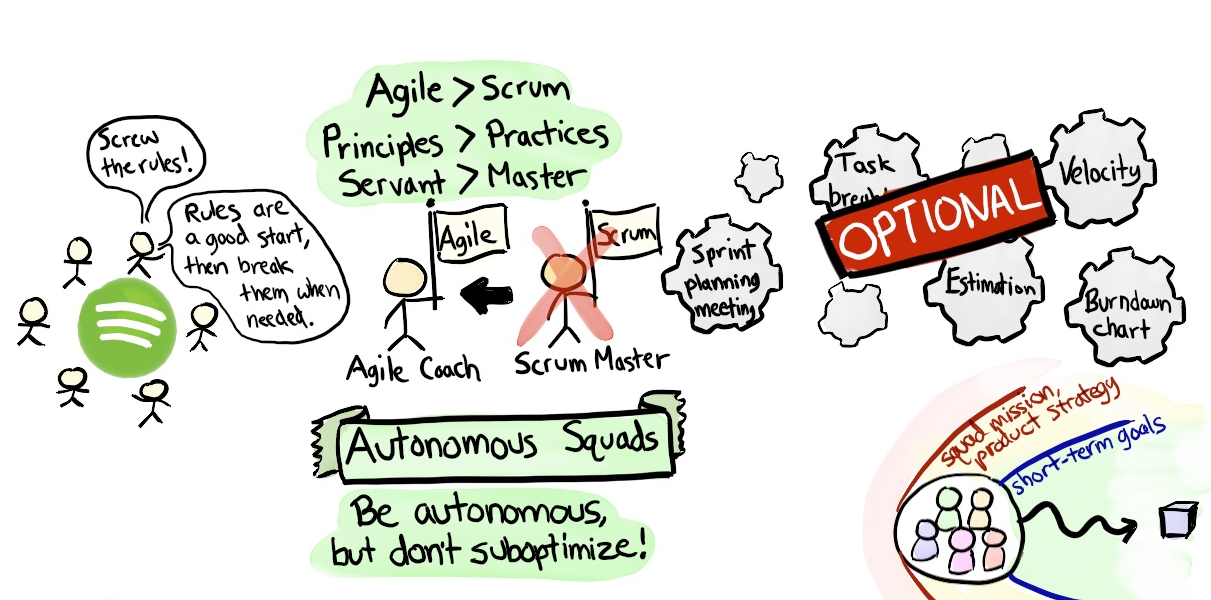
\includegraphics[width=95mm]{./images_spotify/agile_scrum}
\end{center}

Dès ses débuts, Spotify a mis en place une organisation en équipes Scrum, cependant avec la croissance de l'entreprise et la multiplication des équipes, les procédures de Scrum se sont mises à ralentir les équipes.

Partant de l'idée que \textbf{les principes de l'agilité sont plus importants que les pratiques}, les procédures Scrum sont devenues optionnelles et l'organisation des équipes a été chamboulée. Les Scrum Masters sont devenus des coachs Agiles et les équipes Scrum ont été réorganisées en \textbf{Escouades Autonomes}.

Ces escouades sont des équipes \textbf{auto-organisées} --- elles décident de leur organisation interne, de ce qu'elles vont réaliser et de la manière de le réaliser---, \textbf{autonomes et transverses} ---elles sont capables de réaliser une fonctionnalité du début à la fin : conception, développement, tests, déploiement et maintenance--- de moins de huit personnes ayant \textbf{un objectif à long-terme} ---tel que « Faire de Spotify le meilleur endroit pour écouter de la musique » ou « Fournir une infrastructure pour faire du test AB ».

Afin que ces équipes autonomes restent cohérente avec la stratégie de l'entreprise, \textbf{elles sont « alignées » avec la stratégie produit, les priorités de l’entreprise et les autres escouades avec des objectifs à court-terme} négociés tous les trimestres avec leurs supérieurs.

\vspace{5mm}

Pour la direction de Spotify, l'autonomie est extrêmement importante puisqu'ils considèrent qu'elle permet de motiver les employés et que \textbf{des employés motivés construisent de meilleures choses}.

De plus, l'organisation en équipes autonomes réalisant toutes les étapes d'un projet \textbf{permet d'être rapides} en laissant les décisions avoir lieu localement dans l'escouade et de diminuer les transferts de responsabilités à d’autres équipes ---comme lors d'un déploiement réalisé par une autre équipe---, l’attente ou les réunions inter-équipes permettant une mise à l’échelle sans problèmes de dépendances ou de coordination.

Ceci est reflété dans l'architecture de Spotify, organisée en une centaine de micro-services spécialisés, découplés, codés et développés indépendamment. Chacun de ces systèmes appartient à une équipe ---qui en a donc fait la conception, le développement, le déploiement et qui en effectue la maintenance--- et ils sont open-sourcés au sein de Spotify, permettant ainsi à une escouade de soumettre des modifications sur le système d’une autre escouade si cette dernière n’en a pas les capacités. Encore une fois, \textbf{on ne perd pas de temps à attendre que les équipes se coordonnent}.

\newpage

\begin{center}
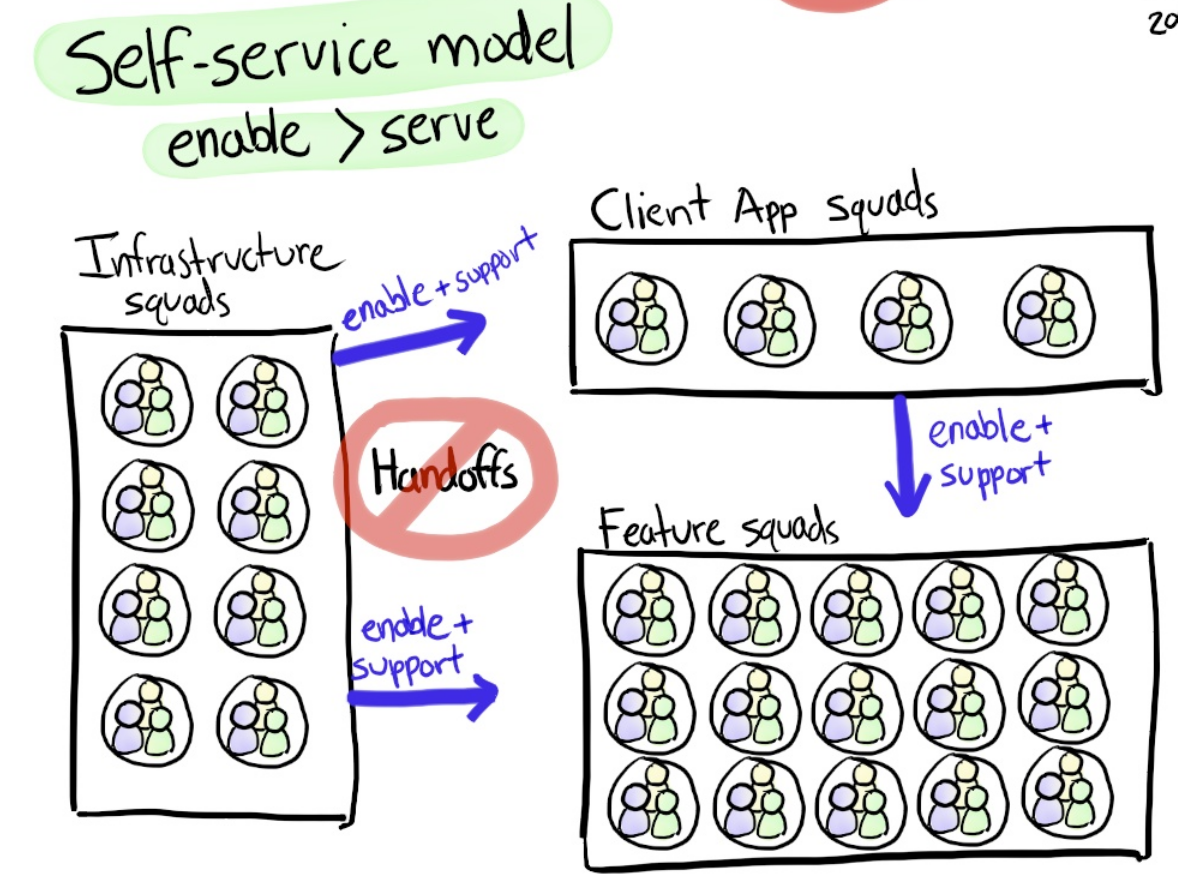
\includegraphics[width=95mm]{./images_spotify/image03}
\end{center}

Ce modèle de « self-service » est aussi appliqué dans les mises en production des fonctionnalités, puisque les escouades sont regroupées en trois types : les escouades s'occupant des clients, les escouades infrastructure et les escouades créant les fonctionnalités.

Le rôle des \textbf{escouades fonctionnalité} est de développer et maintenir toutes les fonctionnalités qu'ils ont à charge (par exemple la recherche de morceaux) sur toutes les plate-formes.

Les \textbf{escouades infrastructure} ont pour objectif de rendre les autres escouades plus efficaces dans leurs mises en production en fournissant des routines et des outils pour la livraison continue, les tests AB et le monitoring.

Les \textbf{escouades clients} quant à elles gèrent un des clients (bureau, web, iOS, Android, etc.) et s'attellent à rendre le déploiement par les autres escouades de nouvelles fonctionnalités au sein de leur client le plus facilement possible.

\newpage

\begin{center}
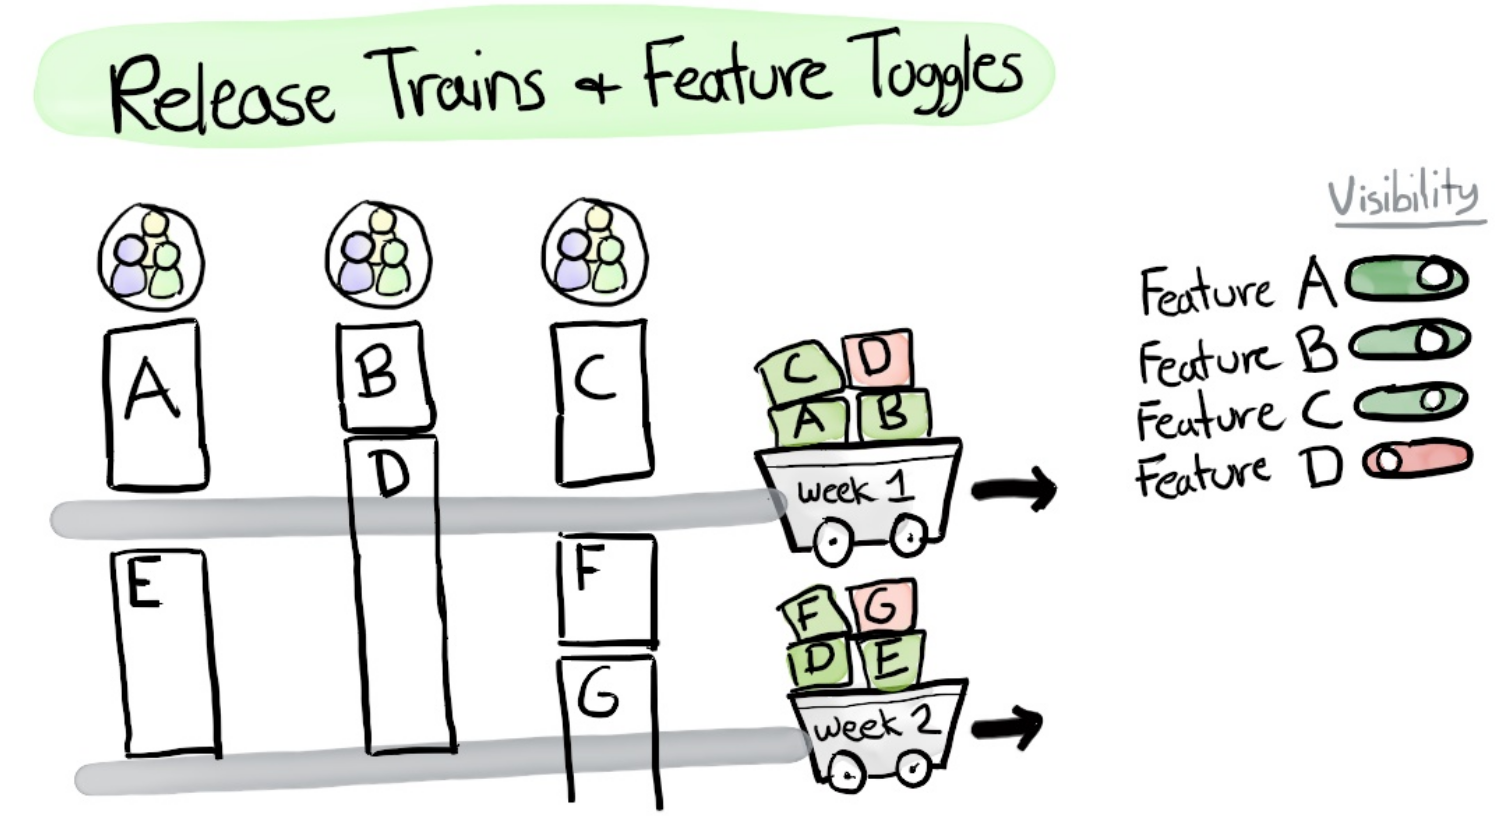
\includegraphics[width=95mm]{./images_spotify/image08}
\end{center}

Ainsi \textbf{Spotify s'efforce de sortir de nouvelles fonctionnalités régulièrement} avec des cycles de release allant de une à trois semaines, et ce même si elles ne sont pas terminées. En effet, chaque fonctionnalité terminées ou en cours de développement est mise en production lorsque le « release train » passe à la fin d'un cycle et les fonctionnalités qui ne sont pas terminées sont masquées avec un « feature toggle ». Ces feature toggle ont plusieurs rôles : masquer les fonctionnalités en cours de développement, tester de nouvelles fonctionnalités en les déployant graduellement aux utilisateurs et masquer des fonctionnalités présentant des erreurs avant qu'elles n'impactent trop d'utilisateurs.

L'architecture découplée et les feature toggles sont importantes dans le processus de création, puisqu'elles permettent de mettre en place \textbf{un environnement dans lequel les développeurs peuvent expérimenter tout en ayant un impact limité en cas d'erreur}. Cet environnement permet également d'encourager les équipes à réaliser plusieurs petites expérimentations et d'en apprendre rapidement, évitant de perdre du temps à prévoir et contrôler les risques en avance.

\newpage

\begin{center}
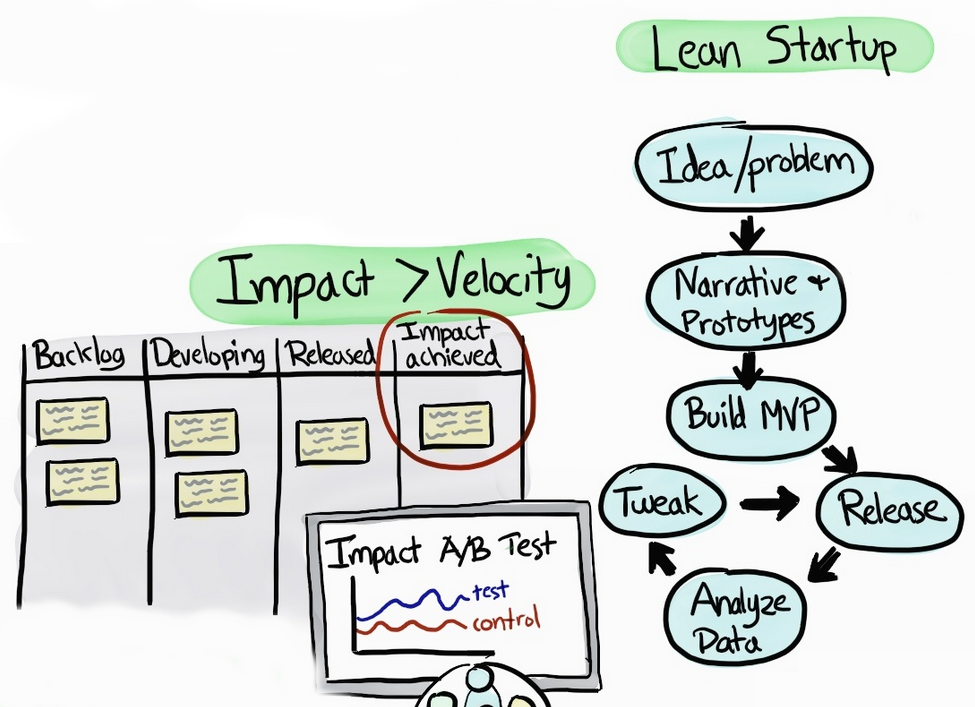
\includegraphics[width=95mm]{./images_spotify/image04}
\end{center}

Le processus de création de fonctionnalité est d'ailleurs \textbf{fondée sur l'expérimentation} : après avoir émit une hypothèse, l'escouade réalise des narratives, des études d'impact puis divers prototypes qui sont testés afin de savoir si les utilisateurs apprécieront la fonctionnalité.

Une fois que l'escouade est confiante dans son idée, elle réalise d’un produit minimum viable qui réalise la narrative mais qui est loin d’être complet. Ce produit minimum viable est par la suite déployé en production et l'escouade réalise des tests A/B afin de tester leur hypothèse. Ces tests sont analysés et la fonctionnalité est ajustée jusqu'à ce que l'impact désiré soit atteint. La fonctionnalité est enfin déployée graduellement au reste des utilisateurs et améliorée par la suite. 

\vspace{5mm}

Il y a une véritable \textbf{culture d'amélioration continue} au sein de Spotify, par le biais de post-mortem et de rétrospectives régulières, mais aussi la mise en place de communautés : 

Chaque employé peut rejoindre une « \textbf{guilde} », une communauté réunissant tous les employés ayant un centre d'intérêt commun tel que le leadership, le  développement web et la livraison continue. Ces guildes sont des lieux d'échanges d'expériences et de bonnes pratiques.

Spotify s'est aperçu qu'\textbf{une organisation autour de communautés fortes permet de se passer d'une structure informelle et volatile} : les escouades sont regroupées en \textbf{tribus} et chaque membre d'une escouade fait partie d'un « \textbf{chapter} », une communauté centrée autour d'une compétence (assistance qualité, coaching agile, développement web, etc.) avec un leader qui coache, mentore ses membres ; leur permettant à l'occasion de changer d'escouade au sein d'une même tribu sans changer de manager.

\section{Netflix : la culture de l'excellence }

\textit{Toutes les informations de cette section proviennent de la présentation de Reed Hastings nommée \texttt{Culture}\supercite{NetflixCultureBook} et de l'article de presse \texttt{How Netflix Reinvented HR}\supercite{NetflixReinventedHR} de Patty McCord, principale investigatrice de la culture d'entreprise de Netflix de 1998 à 2012.} 

\vspace{5mm}

En 2001, l'explosion de la bulle Internet et les attentats du 11 Septembre retardent l'introduction en bourse de Netflix, \textbf{obligeant l'entreprise à se séparer d'un tiers de ses employés}. Quelques mois plus tard en 2002, suite à la popularité des lecteurs DVD durant les fêtes, les services de location de DVD doivent faire face à une demande grandissante ; et \textbf{Netflix se retrouve soudainement avec une charge de travail supplémentaire avec un tiers de ses employés en moins}.

\vspace{5mm}

C'est dans ce contexte que deux conversations vont marquer l'esprit de Patty McCord et définir \textit{la culture Netflix} :

La première est avec un ingénieur qui, suite aux licenciements, se retrouve seul dans son équipe. Il explique que bien qu'il doive travailler plus longtemps, il n'a jamais autant bien travaillé : \textbf{les trois employés qui étaient sous sa responsabilité étaient des employés moyens avec lesquels il perdait beaucoup trop de temps à micro-manager et à corriger leurs erreurs}.

La seconde a lieu avec lieu avec une comptable dont \textbf{les compétences n'étaient plus en adéquation avec les besoins de l'entreprise} après son introduction en bourse. Après lui avoir expliqué qu'ils devaient se séparer d'elle malgré sa longue expérience et sa loyauté envers l'entreprise, l'employée se montre compréhensive et considère le licenciement comme l'occasion de changer de carrière.

\vspace{5mm}

Patty McCord retiendra deux choses de ces entretiens : d'une part que \textbf{des employés « moyens » peuvent freiner les autres}, et d'autre part qu'\textbf{il ne faut pas avoir peur de se séparer d'un employé si il n'est plus indispensable} à l'entreprise. Suite à ça, Netflix va se mettre à \textbf{chercher des employés excellents} et encourager ceux qui ne le sont pas à partir avec des primes de départ généreuses.

Au fil des années, la culture d'entreprise de Netflix s'est articulée afin de permettre d'atteindre l'excellence tant recherchée. 

\vspace{5mm}

Cette excellence est avant tout définie par des \textbf{comportements et compétences promues par Netflix} et recherchées lors des candidatures et des promotions : une capacité de jugement qui soit sage et pragmatique ; de bonnes capacités de communication ; la recherche des meilleurs résultats ; un désir d'apprendre rapidement, de comprendre la stratégie, le marché, les clients et les fournisseurs de l’entreprise ; la création de nouvelles idées innovantes ; la passion, l'honnêteté, la loyauté, le courage et l'altruisme.

Netflix recherche également des employés qui soient \textbf{autonomes et responsables, capables de se discipliner, de s'améliorer, de se motiver et de se comporter en leader}. L'objectif n'est pas seulement de s'entourer des meilleurs talents, mais de \textbf{pouvoir faire fonctionner l’entreprise informellement grâce à l'auto-discipline de chacun}, évitant le chaos induit par la croissance de l'entreprise et l'augmentation de sa complexité tout en permettant une créativité accrue en n'ayant pas à mettre en place des procédures pour tenter de garder le contrôle.

Dans un esprit similaire à celui de Spotify, \textbf{les équipes sont autonomes, transverses et alignées sur les objectifs et la stratégie de l'entreprise}.

\vspace{5mm}

Outre l'autonomie, \textbf{la responsabilité est très valorisée au sein de l'entreprise} : il est attendu des employés qu'ils discutent de leurs problèmes, de leurs compétences et de leurs performances avec leurs supérieurs et collègues, qu'ils gèrent l'argent de Netflix comme le leur, qu'ils gèrent eux-mêmes leurs vacances et qu'ils aient une idée des sources de dépenses et de revenus de l’entreprise afin qu’ils puissent contrôler les dépenses de leurs équipes. 

Brendan Gregg\supercite{WorkingAtNetflix}, ingénieur chez Netflix, considère que cette \textbf{culture de « liberté et responsabilité »} invite les ingénieurs à découvrir et \textbf{proposer de nouvelles solutions, technologies et projets risqués}, pour peu qu'ils soient pertinents et argumentés. 

\section{SpaceX \& Tesla Motors : le culte d'Elon Musk}

\textit{L'essentiel des informations de cette section (ainsi que toutes les autres sections concernant SpaceX et Tesla Motors) proviennent de la biographie \texttt{Elon Musk: Tesla, SpaceX, and the Quest for a Fantastic Future}\supercite{ElonMuskBiography} d'Ashlee Vance, journaliste chez Bloomberg. Les informations restantes proviennent des articles de presse cités dans cette section.} 

\vspace{5mm}

Bien qu'Elon Musk n'ait pas techniquement fondé Tesla Motors, \textbf{il a néanmoins fortement influencé la culture de l'entreprise} dès ses débuts : il a profité de sa popularité auprès de la presse pour être le visage de l'entreprise et il a eu une influence forte sur sa stratégie grâce à son statut d'actionnaire principal.

Son influence sur l'entreprise a par la suite augmenté après que le conseil d'administration ait remercié Eberhard et nommé Ze'ev Drori puis Elon Musk président de Tesla Motors en Octobre 2008\supercite{MuskTeslaCEO}.

Alors qu'aux débuts de SpaceX et Tesla il ait voulu appliquer sa vision jusqu'alors limitée aux projets logiciels (notamment son expérience chez \textit{Zip2} et \textit{X.com}), il a dû réviser ses méthodes de management et les adapter aux contraintes de la production de biens physiques.

\vspace{5mm}

Parmi les méthodes apportées du monde des start-ups, les \textbf{itérations rapides} étaient présentes dès les débuts de la conception du Roadster et de Falcon 1. L'un des principes clés chez Tesla et SpaceX est de pouvoir \textbf{rencontrer rapidement un problème afin de le diagnostiquer et le résoudre le plus tôt possible}.

Pour cela les deux entreprises ont \textbf{massivement recourt aux simulations} : non seulement elles étaient indispensables aux débuts faute de moyens financiers pour réaliser plusieurs prototypes pour les tests, mais elles permettent également de reproduire et corriger des anomalies très rapidement.

\textbf{L'exemple parfait réside dans les bancs de test de SpaceX} sur lequels se trouvent des répliques de l'ensemble des systèmes des fusées Falcon : dès lors qu'une anomalie est détectée sur la fusée durant le lancement, les ingénieurs peuvent la reproduire, réaliser des corrections, les tester sur la réplique puis les envoyer sur la fusée sur le pas de tir \textbf{en seulement quelques heures}, là où la NASA aurait annulé le tir et réalisé un nouvel essai trois semaines plus tard.

\vspace{5mm}

Comme le montre ce recourt aux simulations, une véritable \textbf{chasse au gâchis} a été entreprise par Elon Musk au sein des deux entreprises : \textbf{toute dépense de plus de 10 000 dollars doit être approuvée par ses soins} ---après tout, c'est sa fortune qui est dépensée--- et un \textbf{maximum des pièces sont réalisées en interne}, et ce pour plusieurs raisons.

Tout d'abord parce qu'il \textbf{considère la dépendance aux sous-traitants comme une faiblesse} : non seulement l'entreprise peut se retrouver en difficulté si un sous-traitant les abandonne ou fait faillite, mais \textbf{passer par des intermédiaires fait perdre du temps}.

La seconde raison réside dans les \textbf{besoins spécifiques des deux entreprises} : beaucoup de pièces n'existent pas dans l'industrie ---notamment les moteurs et packs de batteries--- \textbf{ou sont proposées à des tarifs excessifs}, comme celles provenant de l'industrie aérospatiale.

À plusieurs reprises SpaceX a conçu et réalisé des pièces et systèmes \textbf{moins chers, plus compacts et tout aussi performants que leurs équivalents de l'industrie spatiale}, permettant de réaliser de nombreuses économies. Par exemple, les systèmes informatiques des capsules Dragon et des fusées Falcon 9 coûtent près de 10 000 dollars à réaliser contre près de 10 millions de dollars chez la concurrence, tout en réalisant un gain d'espace conséquent dans la capsule Dragon.

Ainsi chez SpaceX \textbf{80 à 90\% des pièces sont réalisées en interne}, là où United Launch Alliance se présente comme un créateur d’emplois en dépendant de près de 1200 fournisseurs différents ; tandis que \textbf{Tesla produit l'intégralité ses Model S et X en trois à cinq jours}.

\vspace{5mm}

SpaceX et Tesla Motors sont dans une \textbf{stratégie d'amélioration continue} : leurs \textbf{usines sont continuellement optimisées} et \textbf{mélangent intelligemment robots et ouvriers} de différents corps de métier. Les premiers ne sont utilisés que pour les tâches très répétitives ou nécessitant une grande précision tandis que les seconds sont employés pour les tâches où l'intelligence humaine est indispensable\supercite{TeslaFactoryPart2}.

Le mélange des corps de métier est une pierre angulaire de SpaceX où \textbf{les ingénieurs côtoient quotidiennement les ouvriers}, les guident et suivent leurs avancées.

\vspace{5mm}

Musk a également poussé les entreprises à utiliser des \textbf{techniques novatrices} telles que le \textit{soudage par friction malaxage}. Alors que les principaux constructeurs de fusées l'évitent au profit des soudures traditionnelles à cause des faiblesses pouvant être introduites par cette technique, Musk a insisté afin que cette technique soit perfectionnée et utilisée au sein de SpaceX. 

Le pari en valait la peine puisque la technique leur a permis d'utiliser des alliages plus légers et de se passer de rivets et de structures de soutiens, résultant en des \textbf{gains de poids conséquents}. La méthode a depuis été transférée à Tesla et commence à être \textbf{imitée par ses concurrents} ---notamment \textit{Blue Origin} qui a débauché l'un des ingénieurs ayant mis au point la technique.

\vspace{5mm}

Une chose que Musk a cependant gardé intact de l'esprit start-up de ses débuts est la \textbf{recherche continue des meilleurs talents}. Pour cela ses entreprises n'hésitent pas à approcher les universités afin de recruter directement les étudiants les plus brillants ou encore à inviter certains participants d'une convention à un entretien privé dans un bar ou restaurant proche.

Musk recherche des\textbf{ esprits brillants et passionnés} capables de résoudre des problèmes concrets et \textbf{ayant une expérience manuelle} telle que la participation à un concours de robotique ou la construction d'un véhicule électrique sur leur temps libre.

Les premiers entretiens se concentrent sur le parcours et la motivation des candidats tandis que les suivants se déroulent avec les managers et les futurs collègues afin de s'assurer qu'il s'intégrera correctement à l'équipe. Pour les postes les plus techniques il leur sera demandé de \textbf{diagnostiquer des problèmes concrets et de trouver une solution}, de réaliser un programme de plusieurs milliers de lignes en quelques heures ou encore d'analyser des données sans instructions.

Pour SpaceX ces postes à haut niveau doivent passer une étape supplémentaire : ils doivent \textbf{rédiger une dissertation sur leurs motivations à destination d'Elon Musk}, qui les conviera à un entretien final. Durant cet entretien Musk a pour habitude de poser une énigme aux candidats. L'exactitude de la réponse importe peu, il \textbf{s'intéresse avant tout au raisonnement} qu'ont eu les candidats.

\vspace{5mm}

Avec des employés si motivés et talentueux, les entreprises se permettent de \textbf{maximiser le pouvoir des individus}. Elles partent du principe qu'un individu prêt à abattre une masse incroyable de travail peut réaliser plus de travail qu'un groupe, puisqu'il ne perd pas de temps à être interrompu, à obtenir le consensus ou à organiser des réunions.

Cependant \textbf{ce rythme de travail est loin de convenir à tous} ---les ingénieurs travaillent souvent près de douze heures par jour---, d'autant plus que les \textbf{ingénieurs sont laissés en autonomie} et que Musk attend d'eux qu'ils soient capable d'abattre autant de travail que lui ---il est réputé pour avoir une endurance sans commune mesure et d'être capable de travailler plus de trois jours de suite sans jamais s'arrêter ni dormir---, amenant certains à quitter l'entreprise quelques semaines après leur embauche. 